

\section{Problem Formulation}
\label{sec:problem-formulation}


\textbf{Star Quantum Network.}To ease the presentation, let us first consider  a  three-link star quantum network, illustrated in
Fig.~\ref{fig:three-link-star}, is represented by a graph
\(\mathcal G\coloneqq(\mathcal N,\mathcal L)\), where
\(\mathcal N\) denotes the set of nodes and
\(\mathcal L\) denotes the set of quantum links connecting them.
We model each quantum link as a Pauli channel. Note that more general quantum
channels can be converted into effective Pauli channels through
Pauli twirling
\cite{PhysRevA.72.052326,PhysRevA.54.3824}.

Here, \(C\)  is the central node while
\(N_1,N_2,N_3\) are peripheral nodes, as illustrated in
Fig.~\ref{fig:three-link-star}.
Each peripheral node $N_\ell$ is connected to the central node $C$ through one
quantum link which is described by a Pauli channel with unknown channel parameters,
\begin{equation}
    \mathcal P_\ell(\!\sigma\!)
    {=}
    A_\ell\sigma
    {+}B_\ell X\sigma X
        {+}C_\ell Y\sigma Y
        {+}D_\ell Z\sigma Z,
\ell {\in}\{\!1,2,3\!\},
    \label{eq:link-pauli-channel}
\end{equation}
where parameters \(A_\ell ,B_\ell ,C_\ell ,D_\ell \geq0\) and
\(A_\ell +B_\ell +C_\ell +D_\ell =1\).
Its nontrivial PTM eigenvalues
\(q_{X,\ell },q_{Y,\ell },q_{Z,\ell }\) are defined in~\eqref{eq:pauli-channel-ptm}.
Each link is therefore completely characterized by either
\((A_\ell,B_\ell,C_\ell,D_\ell)\) or
\((q_{X,\ell},q_{Y,\ell},q_{Z,\ell})\).
We  impose the following nonzero condition on the
link channels to simplify the estimation analysis by excluding
degenerate cases\footnote{This condition is sufficient
    for the proposed estimation but is not necessary for
    identifiability. If
    $q_{X,\ell}=q_{Y,\ell}=q_{Z,\ell}=0$, then
    $\mathcal P_\ell$ is completely depolarizing and
    $(\mathcal I\otimes\mathcal P_\ell)(\rho)=I\otimes I/4$ for every
    Bell-diagonal state $\rho$ \cite{gottesman2026surviving}. Such a link erases all correlations and can
    be treated as a failed link using existing link-failure identification
    methods~\cite{inproceedings,10.1007/978-3-540-24668-8_19}. If only some PTM
    eigenvalues vanish, the Clifford dressings in
    \S\ref{subsec:Clifford-dressing} can permute the zero and nonzero
    entries. Alternative configurations may then recover the remaining
    parameters whenever sufficiently many nonsingular product equations
    are available. A complete analysis of these degenerate cases is beyond
    the scope of this paper.}.
\begin{assumption}[Nonzero PTM eigenvalues]
    \label{ass:nonzero-eigenvalues}
    For every link \(\ell\in\{1,2,3\}\), all nontrivial PTM
    eigenvalues are nonzero:
    \begin{equation}
        q_{P,\ell}\neq 0,
        \qquad
        P\in\{X,Y,Z\},\quad \ell\in\{1,2,3\}.
    \end{equation}
\end{assumption}




\textbf{Peripheral Monitors and End-to-End Access.}
The peripheral nodes \(N_1,N_2,N_3\), referred to as
\emph{monitors}
, provide the state preparation and measurement
(SPAM) capabilities used for tomography.
The central node \(C\) can route quantum systems, perform prescribed
local operations, including quantum gates \(S\), \(H\), and controlled-NOT (CNOT) gates,
and discard auxiliary qubits. However, its SPAM capabilities, if
present, are inaccessible to the tomography procedure.

We emphasis that this access model follows the end-to-end monitoring framework
in the classical network tomography literature and is also adopted
in quantum network tomography~\cite{wang2025quantumnetworktomographygeneral,
    He_Ma_Swami_Towsley_2021}.
It also reflects practical scenarios in which peripheral nodes
are accessible to users, whereas the central node is managed by
a quantum network service provider that permits prescribed operations but does
not grant users access to its internal SPAM capabilities or
measurement records.






% Insert Fig.~\ref{fig:three-link-star} here.

\begin{figure}[tb]
    \centering
    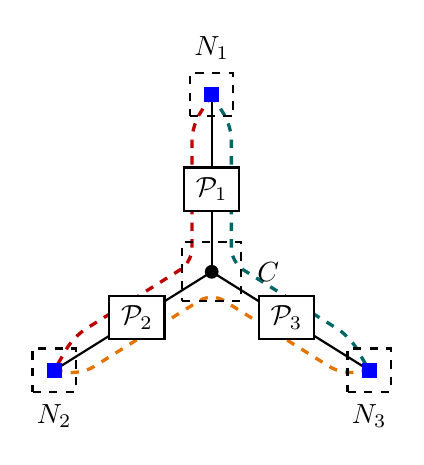
\begin{tikzpicture}[
            line/.style={thick},
            proc/.style={
                    rectangle, draw, fill=white, thick,
                    minimum width=0.7cm,
                    minimum height=0.55cm,
                    inner sep=1pt
                },
            endpoint/.style={
                    rectangle, fill=blue, draw=blue,
                    minimum size=0.18cm, inner sep=0pt
                },
            station/.style={
                    rectangle, draw, dashed, thick,
                    minimum width=0.55cm,
                    minimum height=0.55cm
                },
            center/.style={
                    circle, fill=black, draw=black,
                    minimum size=0.16cm, inner sep=0pt
                },
            pathline/.style={
                    very thick, dashed, rounded corners=5pt
                }
        ]
        \coordinate (C)  at (0,0);
        \coordinate (A1) at (0,2.25);
        \coordinate (A2) at (-2.0,-1.25);
        \coordinate (A3) at (2.0,-1.25);

        % Physical links
        \draw[line] (A1) -- (C);
        \draw[line] (A2) -- (C);
        \draw[line] (A3) -- (C);

        % Three end-to-end paths, offset for visual clarity
        \draw[pathline,red!75!black]
        (A1) -- (-0.25,1.85) -- (-0.25,0.12)
        -- (-1.75,-0.82) -- (A2);

        \draw[pathline,teal!80!black]
        (A1) -- (0.25,1.85) -- (0.25,0.12)
        -- (1.75,-0.82) -- (A3);

        \draw[pathline,orange!90!black]
        (A2) -- (-1.65,-1.30) -- (0,-0.27)
        -- (1.65,-1.30) -- (A3);

        % Pauli channels
        \node[proc] (P1) at (0,1.05) {$\mathcal P_1$};
        \node[proc] (P2) at (-0.95,-0.58) {$\mathcal P_2$};
        \node[proc] (P3) at (0.95,-0.58) {$\mathcal P_3$};

        % Central node
        \node[station,minimum width=0.75cm,
            minimum height=0.75cm] at (C) {};
        \node[center] at (C) {};
        \node[right=13pt] at (C) {$C$};

        % Peripheral monitors
        \node[station] at (A1) {};
        \node[endpoint] at (A1) {};
        \node[above=9pt] at (A1) {$N_1$};

        \node[station] at (A2) {};
        \node[endpoint] at (A2) {};
        \node[below=9pt] at (A2) {$N_2$};

        \node[station] at (A3) {};
        \node[endpoint] at (A3) {};
        \node[below=9pt] at (A3) {$N_3$};



    \end{tikzpicture}
    \caption{ Three-link star network with peripheral monitors \(N_1,N_2,N_3\) (blue squares) and a central node \(C\) (black circle). Each link \(\ell\) is modeled by an unknown Pauli channel \(\mathcal P_\ell \). The monitors provide SPAM capabilities, while \(C\) performs prescribed operations without supplying measurement outcomes to the tomography procedure. The red, teal, and orange dashed lines represent the three end-to-end paths
0        $N_1\!-\!C\!-\!N_2$, $N_1\!-\!C\!-\!N_3$, and $N_2\!-\!C\!-\!N_3$, respectively. }
    \label{fig:three-link-star}
\end{figure}


\textbf{End-to-End Distillation.}
Under the access constraints described above, we consider only
end-to-end (path-level) entanglement distillation between monitors. The local measurements required at both endpoints
by distillation protocols  can then be performed at the
monitors, with their outcomes accessible to the tomography procedure.
Link-level distillation would instead involve measurements at \(C\),
whose outcomes are unavailable to users. Even if the service provider
performs such distillation internally, we exclude it from our model
and use only measurement data obtained from path-level distillation. Specifically, we apply the double-selection protocol described in
\S~\ref{doub} to entangled pairs shared between monitors.
Besides conditionally retaining an output pair, the protocol
provides measurement statistics for estimating the input Bell-diagonal state.

We use these statistics in two estimation schemes.
Under the fidelity condition $F(\rho)>1/2$,
Lemma~\ref{lem:double-selection-statistics} allows all three
nontrivial parameters to be estimated using
\eqref{eq:double-selection-inversion}.
Alternatively, Observation~\ref{lem3} allows the $Z$-basis parameters
to be estimated from $p_Z$ alone without relying on this fidelity condition.
Suitable Clifford dressings extend the latter approach to
the $X$ and $Y$ components.
In both schemes, the estimated end-to-end correlations are
then combined to infer the individual link-level channel parameters.

The following assumption ensures the applicability of
Lemma~\ref{lem:double-selection-statistics} to  JCE.
Note that it is not required by MCE, which is based on
Observation~\ref{lem3}.

\begin{assumption}[Fidelity condition for JCE]
    \label{ass:fidelity-condition}
    The Bell-diagonal states
    $\rho_{12}$, $\rho_{13}$, $\rho_{\text{m},23}$, and
    $\rho_{\text{d},23}$, defined in
    \eqref{eq:direct-two-link-states},
    \eqref{eq:mergecast-undressed-state}, and
    \eqref{eq:mergecast-dressed-state}, each have fidelity greater
    than $1/2$ with respect to $\ket{\Phi^+}$.
\end{assumption}


\textbf{Objective.}
Given the three-link star network
\(\mathcal G\), our objective is to design end-to-end protocols that use distillation
measurement outcomes to estimate all link-level channel parameters
\(q_{P,\ell}\), for \(\ell\in\{1,2,3\}\) and
\(P\in\{X,Y,Z\}\). We quantify the estimation accuracy using the mean square error (MSE),
\begin{equation}
    \epsilon_{\mathrm{est}}
    \coloneqq
        \frac{1}{9}
        \sum_{\ell=1}^{3}
        \sum_{P\in\{X,Y,Z\}}
        \left(
        \widehat{q}_{P,\ell}-q_{P,\ell}
        \right)^2
    ,
\end{equation}
where \(\widehat{q}_{P,\ell}\) denotes the estimate of \(q_{P,\ell}\).
Our objective is to minimize this estimation error for a given measurement budget.
\begin{remark}[Extension to general network topologies]
    \label{rem:general-topology}
    Due to space limitations, this work focuses on the three-link star
    topology, which provides a fundamental setting in which individual
    link parameters can be estimated from end-to-end observations
    without access to the central node's measurement outcomes.

    The proposed framework can be naturally extended to more general
    quantum-network topologies without degree-two nodes based on two
    observations. First, any quantum network without degree-two nodes can
    be viewed as being composed of three-link star substructures. Second,
    for tomography purposes, two consecutive Pauli channels can be
    regarded as a single effective Pauli channel. We illustrate this
    extension through a larger-network example in \S~\ref{sub2}.
    A more comprehensive treatment is omitted due to space limitations.
\end{remark}
